\input format.tex

\usepackage{graphicx}
\graphicspath{{cores/}}

\begin{document}

\vspace*{6mm}
%% 各章节
\setlength{\arrayrulewidth}{1pt}
\fontsize{9.3pt}{11pt}\selectfont
\color{gray2}

\begin{spacing}{1.5}
\begin{LRaside}[.8]{1.2有益菌与有害菌}
\noindent

\includegraphics[width=\linewidth]{youyiyouhaijun.pdf}
\asidebreak %
有益菌,指对人类有益的细菌。它们是肠道里的“正义卫士”,不仅能够产生维生素等有益物质,还能抵御致病菌的入侵,减少炎症。有害菌,是肠道里的“捣蛋鬼”,产生毒素等有害物质。有害菌在肠道内数量较少,一般情况下不会对人体健康产生大的影响,但一旦肠道菌群平衡失调,有害菌异常大量增殖,就可能引发多种健康问题。
\end{LRaside}
\end{spacing}

\vspace*{5mm}

\begin{minipage}[t]{.47\textwidth}
{\bf 有益菌}
\vspace{8pt}


\includegraphics[width=1.3cm]{youyijun_1.pdf}~~

\includegraphics[width=1.3cm]{youyijun_2.pdf}~~

\includegraphics[width=1.3cm]{youyijun_3.pdf}

\smallskip

\fontsize{8}{13}\selectfont
\begin{tikzpicture}[scale=1.8,x=1.0cm,y=1.0cm, declare function={
filltop1=11.62;
filltop2=0.22;
fillper=0.0677;}]

\pgfmathparse{{filltop1}}\let\pgfmathresultfilltopa\pgfmathresult
\pgfmathparse{{filltop2}}\let\pgfmathresultfilltopb\pgfmathresult
\pgfmathparse{{fillper}}\let\pgfmathresultfillper\pgfmathresult

\def\filltopa{\pgfmathresultfilltopa}
\def\filltopb{\pgfmathresultfilltopb}
\def\fillpercent{\pgfmathresultfillper}

\pgfmathsetmacro{\filltopaa}{15};

% 直接根据分布求得百分比计算检测值长条覆盖的比例
\pgfmathsetmacro{\filltopbb}{\fillpercent*30};

% 根据均值与检测的比例检测值长条覆盖的比例
%\pgfmathparse{\filltopb/\filltopa}\let\pgfmathswitch\pgfmathresult

%\pgfmathtruncatemacro\one{\pgfmathswitch}
%\pgfmathtruncatemacro\two{2}
%\ifnum\one>\two
%\pgfmathsetmacro{\filltopbb}{30};
%\fi
%\ifnum\one=\two
%\pgfmathsetmacro{\filltopbb}{30};
%\fi
%\ifnum\one<\two
%\pgfmathsetmacro{\filltopbb}{\pgfmathswitch*15};
%\fi

\begin{scope}

\draw[fill=gray1,color=gray1,very thick] (0,0) -- (30mm,0) -- (30mm,2.8mm) -- (0,2.8mm);
\path (0,1.4mm) node [yshift=1.5mm,left=0mm] {平均};
\path (0,1.4mm) node [yshift=-1.5mm,left=0mm] {指数};


\draw[fill=topcolor2,color=topcolor2,very thick] (0,0) -- (\filltopaa*1mm,0) -- (\filltopaa*1mm,2.8mm) -- (0,2.8mm);
\path (30mm,1.4mm) node [right=0mm] {\filltopa};
\end{scope}


\begin{scope}[yshift=-5mm]
\draw[fill=gray1,color=gray1,very thick] (0,0) -- (30mm,0) -- (30mm,2.8mm) -- (0,2.8mm);
\path (0,1.4mm) node [yshift=1.5mm,left=0mm] {您的};
\path (0,1.4mm) node [yshift=-1.5mm,left=0mm] {指数};


\draw[fill=topcolor2,color=topcolor2,very thick] (0,0) -- (\filltopbb*1mm,0) -- (\filltopbb*1mm,2.8mm) -- (0,2.8mm);
\path (30mm,1.4mm) node [right=0mm] {\filltopb};
\end{scope}

\end{tikzpicture}
\begin{center}

\includegraphics[width=.35cm]{xiaoren07.pdf}
\pdfchatu{xiaoren0}{9}

\textbf{\small 您的有益菌含量高于6.77{\%}的参考人群 }
\end{center}
\end{minipage}
\hfill
\begin{minipage}[t]{.47\textwidth}
{\bf 有害菌}
\vspace{8pt}


\includegraphics[width=1.3cm]{youhaijun_1.pdf}~~

\includegraphics[width=1.3cm]{youhaijun_2.pdf}~~

\includegraphics[width=1.3cm]{youhaijun_3.pdf}

\smallskip

\fontsize{8}{13}\selectfont
\begin{tikzpicture}[scale=1.8,x=1.0cm,y=1.0cm, declare function={
filltop1=5.57;
filltop2=0.28;
fillper=0.2747;}]

\pgfmathparse{{filltop1}}\let\pgfmathresultfilltopa\pgfmathresult
\pgfmathparse{{filltop2}}\let\pgfmathresultfilltopb\pgfmathresult
\pgfmathparse{{fillper}}\let\pgfmathresultfillper\pgfmathresult

\def\filltopa{\pgfmathresultfilltopa}
\def\filltopb{\pgfmathresultfilltopb}
\def\fillpercent{\pgfmathresultfillper}

\pgfmathsetmacro{\filltopaa}{15};

% 直接根据分布求得百分比计算检测值长条覆盖的比例
\pgfmathsetmacro{\filltopbb}{\fillpercent*30};

% 根据均值与检测的比例检测值长条覆盖的比例
%\pgfmathparse{\filltopb/\filltopa}\let\pgfmathswitch\pgfmathresult

%\pgfmathtruncatemacro\one{\pgfmathswitch}
%\pgfmathtruncatemacro\two{2}
%\ifnum\one>\two
%\pgfmathsetmacro{\filltopbb}{30};
%\fi
%\ifnum\one=\two
%\pgfmathsetmacro{\filltopbb}{30};
%\fi
%\ifnum\one<\two
%\pgfmathsetmacro{\filltopbb}{\pgfmathswitch*15};
%\fi

\begin{scope}

\draw[fill=gray1,color=gray1,very thick] (0,0) -- (30mm,0) -- (30mm,2.8mm) -- (0,2.8mm);
\path (0,1.4mm) node [yshift=1.5mm,left=0mm] {平均};
\path (0,1.4mm) node [yshift=-1.5mm,left=0mm] {指数};


\draw[fill=yellow2,color=yellow2,very thick] (0,0) -- (\filltopaa*1mm,0) -- (\filltopaa*1mm,2.8mm) -- (0,2.8mm);
\path (30mm,1.4mm) node [right=0mm] {\filltopa};
\end{scope}


\begin{scope}[yshift=-5mm]
\draw[fill=gray1,color=gray1,very thick] (0,0) -- (30mm,0) -- (30mm,2.8mm) -- (0,2.8mm);
\path (0,1.4mm) node [yshift=1.5mm,left=0mm] {您的};
\path (0,1.4mm) node [yshift=-1.5mm,left=0mm] {指数};


\draw[fill=yellow2,color=yellow2,very thick] (0,0) -- (\filltopbb*1mm,0) -- (\filltopbb*1mm,2.8mm) -- (0,2.8mm);
\path (30mm,1.4mm) node [right=0mm] {\filltopb};
\end{scope}

\end{tikzpicture}

\begin{center}
\pdfchatuorange{xiaoren1}{2}
\includegraphics[width=.35cm]{xiaoren17.pdf}
\pdfchatu{xiaoren1}{7}

\textbf{\small 您的有害菌含量高于27.47{\%}的参考人群}
\end{center}
\end{minipage}

\vspace*{3mm}

{\qihao 平均指数:表示健康人群中有益菌、有害菌的平均值。}

\vspace*{8mm}

\begin{spacing}{1.5}
\begin{LRaside}[.8]{结果分析}
\noindent
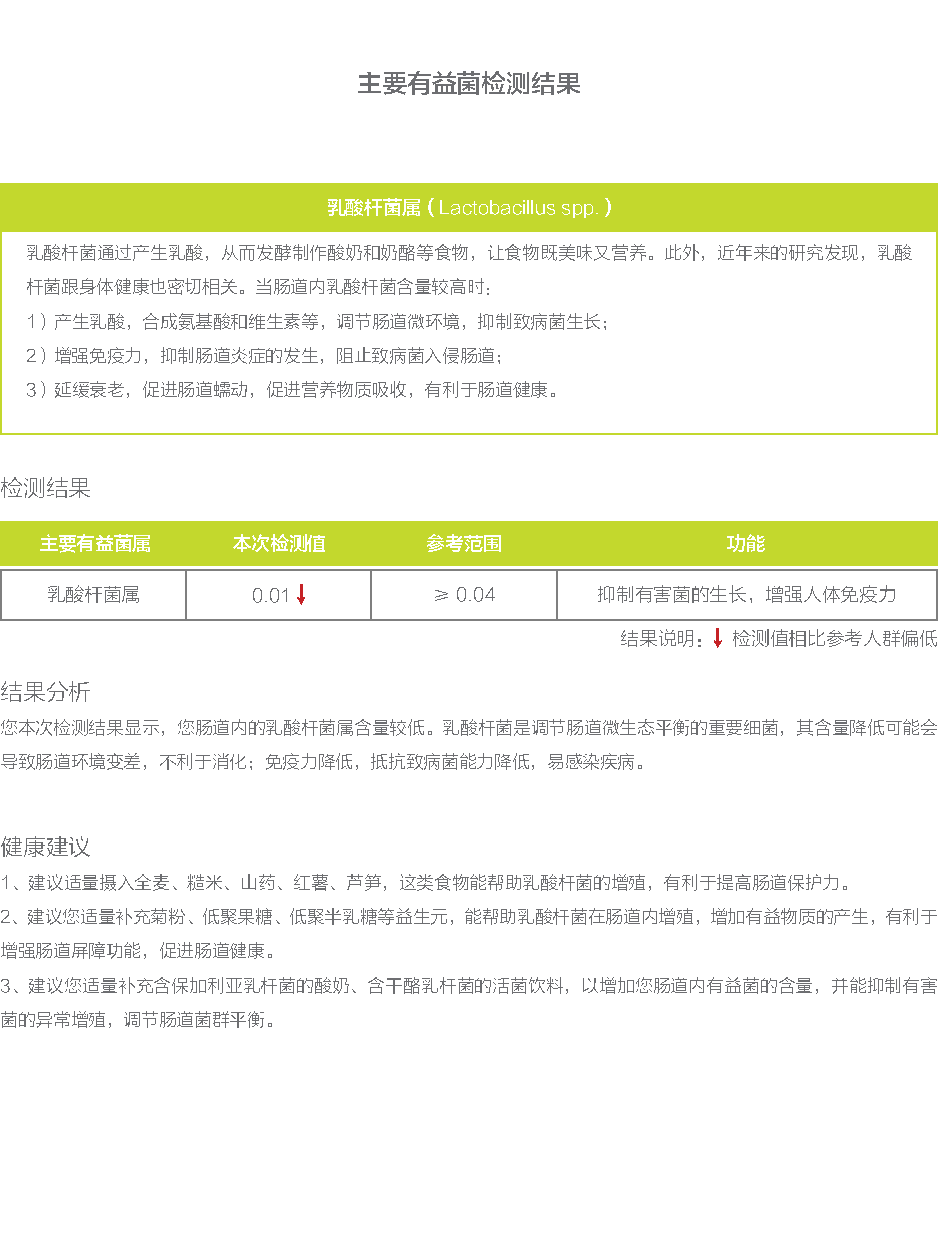
\includegraphics[width=\linewidth]{result.pdf}
\asidebreak %
您肠道内的有害菌含量偏高,会产生毒素等有害物质,可能会引起口臭、感染、腹泻、肠炎、便秘等。有害菌数量过高还可能影响您的心情和食欲,扰乱内分泌,降低机体免疫力,增加疾病风险。但同时您肠道内的有益菌含量也较高,数量较多的有益菌能够起到拮抗作用,降低有害菌可能对您造成的危害。有害菌在您免疫力低下时,可能导致相关疾病,建议您规律作息,注意饮食健康,预防潜在的健康风险。
\end{LRaside}
\end{spacing}

\end{document}
